\section*{Cycle 2 Experiment 11}

\section{\Large{Simple Mail Transfer Protocol}}

\subsection{Aim}
\large To implement simulation of SMTP(Simple Mail transfer Protocol) using UDP.

\subsection{Theory}
SMTP is part of the application layer of the TCP/IP protocol. Using a process called ”store and forward,” SMTP moves your email on and across networks. SMTP makes use of a set of commands to transfer information via the client and server. Some of the important ones include:
\begin{itemize}
    \item HELO: The HELO command is used to initiate an SMTP session.
    \item MAIL FROM: command is used primarily to send email addresses, it needs a way to alert the recipient host to who is sending the inbound message.
    \item RCPT TO: command tells the receiving host the email address of the message recipient
    \item DATA: When the sending host transmits the DATA command, it tells the receiving host that a stream of data will follow. End the data stream with <CRLF >.<CRLF >
    \item QUIT: QUIT command is used to terminate an SMTP session.
\end{itemize}
Based on similar information regarding SMTP, the basic intent here is to simulate how SMTP works to move your mail on and across networks.
\subsection{Algorithm}
\begin{verbatim}
Algorithm for the Server

1 START
2 Define the registered users
3 Define the domain
4 Create the socket using socket()
5 Configure sockaddr_in, the structure describing an Internet Socket Address
6 Bind the address struct to the socket using bind()
7 Listen to the socket
8 A new socket for the incoming connection is created using accept()
9 Send the message with status 220 to denote that it is ready
10 If client's reply HELO command, server responds with status '250 ok' message. 
11 If the response contain a 'from mail' that is registered in the server, 
    status 250 is returned. 
12 If the response contain a 'to mail' that is registered in the server, status 
    250 is returned.
13 If the reply contains 'DATA' command, server responds with 354 to start 
    mail input
14 The received body is written onto a file with from mail
15 If QUIT is received, '221 service closing' is returned to client
16 Close the socket
17 STOP

Algorithm for the Client

1 START
2 Get the from and to mail addresses
3 Create the socket using socket()
4 Configure sockaddr_in, the structure describing an Internet Socket Address
5 Connect to the server using connect()
6 If 220 status is returned from the server, connection is established 
    successfully
7 Send 'HELO' command to the server
8 If the response contains 250, HELO successful
9 Send the mail to the server (MAIL FROM)
10 If the response is 250, the user is registered
11 Send the mail to the server(RCPT TP). If the response is 250, the user
    is registered
12 Send DATA command to the server. If status received is 354, goto step 13
13 Send the body of the mail to the server
14 To quit the connection, sent the command QUIT
15 If response is 221, connection is closed with the server
16 Close the socket
17 STOP
\end{verbatim}

\subsection{Program \& Output}
\begin{verbatim}
//Simple Mail Transfer Protocol using UDP
//Server side

#include <stdio.h>
#include <string.h>
#include <sys/socket.h>
#include <sys/types.h>
#include <netinet/in.h>
#include <arpa/inet.h>
#include <fcntl.h>
#include <stdlib.h>

#define MAXLINE 100
main(int argc, char *argv[])
{
    int n, sock_fd;
    struct sockaddr_in servaddr, cliaddr;
    char mesg[MAXLINE + 1];
    socklen_t len;
    char *str_ptr, *buf_ptr, *str;
    len = sizeof(cliaddr);
    if ((sock_fd = socket(AF_INET, SOCK_DGRAM, 0)) < 0)
    {
        printf("SOCKET NOT CREATED\n");
        exit(1);
    }
    bzero((char *)&servaddr, sizeof(servaddr));

    servaddr.sin_family = AF_INET;
    servaddr.sin_port = htons(atoi(argv[1]));
    servaddr.sin_addr.s_addr = htonl(INADDR_ANY);

    if (bind(sock_fd, (struct sockaddr *)&servaddr, sizeof(servaddr)) < 0)
    {
        perror("BIND FAILED");
        exit(1);
    }
    if((n=recvfrom(sock_fd,mesg,MAXLINE,0,(struct sockaddr*)&cliaddr,&len))== -1)
    {
        perror("size not received:");
        exit(1);
    }
    mesg[n] = '\0';
    printf("%s\n", mesg);
    sprintf(mesg, "220 from_server_mail_server\n");

    sendto(sock_fd, mesg, MAXLINE, 0,(struct sockaddr*)&cliaddr, sizeof(cliaddr));
    n = recvfrom(sock_fd, mesg, MAXLINE, 0, (struct sockaddr *)&cliaddr, &len);

    mesg[n] = '\0';
    printf("C:%s\n", mesg);
    str_ptr = strdup(mesg);
    buf_ptr = strsep(&str_ptr, " ");
    sprintf(mesg, "250 HELO %s", str_ptr);
    free(buf_ptr);

    sendto(sock_fd, mesg, MAXLINE, 0,(struct sockaddr*)&cliaddr, sizeof(cliaddr));
    n = recvfrom(sock_fd, mesg, MAXLINE, 0, (struct sockaddr *)&cliaddr, &len);

    mesg[n] = '\0';
    printf("C: %s", mesg);
    str_ptr = strdup(mesg);
    buf_ptr = strsep(&str_ptr, ":");
    str_ptr[strlen(str_ptr) - 1] = '\0';
    sprintf(mesg, "250 HELO %s.......Sender OK\n", str_ptr);
    free(buf_ptr);

    sendto(sock_fd, mesg, MAXLINE, 0,(struct sockaddr*)&cliaddr, sizeof(cliaddr));
    n = recvfrom(sock_fd, mesg, MAXLINE, 0, (struct sockaddr *)&cliaddr, &len);

    mesg[n] = '\0';
    printf("C: %s", mesg);
    str_ptr = strdup(mesg);
    buf_ptr = strsep(&str_ptr, ":");
    str_ptr[strlen(str_ptr) - 1] = '\0';
    sprintf(mesg, "250 HELO %s.......Recepient OK\n", str_ptr);
    free(buf_ptr);

    sendto(sock_fd, mesg, MAXLINE, 0,(struct sockaddr*)&cliaddr, sizeof(cliaddr));
    n = recvfrom(sock_fd, mesg, MAXLINE, 0, (struct sockaddr *)&cliaddr, &len);
    mesg[n] = '\0';
    printf("C: %s\n", mesg);
    sprintf(mesg, "354 Enter body of mail. End with \".\" on a newline\n");
    sendto(sock_fd, mesg, MAXLINE, 0,(struct sockaddr*)&cliaddr, sizeof(cliaddr));
    while (1)
    {
        n = recvfrom(sock_fd, mesg, MAXLINE, 0, (struct sockaddr *)&cliaddr, &len);
        mesg[n] = '\0';
        printf("C: %s\n", mesg);
        mesg[strlen(mesg) - 1] = '\0';

        str = mesg;
        while (isspace(*str++))
            ;
        if (strcmp(--str, ".") == 0)
            break;
        sprintf(mesg, "250 Messages accepted for delivery \n");
        sendto(sock_fd, mesg, MAXLINE, 0, (struct sockaddr *)&cliaddr, 
            sizeof(cliaddr));
        n = recvfrom(sock_fd, mesg, MAXLINE, 0, (struct sockaddr*)&cliaddr, &len);
        mesg[n] = '\0';
        printf("C: %s\n", mesg);
        sprintf(mesg, "221 Mail server closing connection\n");
        sendto(sock_fd, mesg, MAXLINE, 0, (struct sockaddr *)&cliaddr, 
            sizeof(cliaddr));
    }
}

//Client side

#include <stdio.h>
#include <string.h>
#include <sys/socket.h>
#include <sys/types.h>
#include <netinet/in.h>
#include <arpa/inet.h>
#include <fcntl.h>
#include <stdlib.h>

#define MAXLINE 100
main(int argc, char *argv[])
{
    int n;
    int sock_fd;
    int i = 0;
    struct sockaddr_in servaddr;
    char buf[MAXLINE + 1];

    char address_buf[MAXLINE], message_buf[MAXLINE];
    char *str_ptr, *buf_ptr, *str;
    if (argc != 3)
    {
        fprintf(stderr, "Command is :./SMTPclient <address_port>\n");
        exit(1);
    }
    if ((sock_fd = socket(AF_INET, SOCK_DGRAM, 0)) < 0)
    {
        printf("SOCKET NOT CREATED\n");
        exit(1);
    }
    bzero((char *)&servaddr, sizeof(servaddr));
    servaddr.sin_family = AF_INET;
    servaddr.sin_port = htons(atoi(argv[2]));
    inet_pton(AF_INET, argv[1], &servaddr.sin_addr);
    sprintf(buf, "SMTP REQUEST FROM CLIENT\n");

    n = sendto(sock_fd, buf, strlen(buf), 0, (struct sockaddr *)&servaddr, 
        sizeof(servaddr));
    if (n < 0)
    {
        perror("ERROR");
        exit(1);
    }

    if ((n = recvfrom(sock_fd, buf, MAXLINE, 0, NULL, NULL)) == -1)
    {
        perror("UDP READ ERROR");
        exit(1);
    }
    buf[n] = '\0';
    printf("S: %s", buf);
    sprintf(buf, "HELO from_client_mail_server\n");

    n = sendto(sock_fd, buf, strlen(buf), 0, (struct sockaddr *)&servaddr, 
        sizeof(servaddr));

    if ((n = recvfrom(sock_fd, buf, MAXLINE, 0, NULL, NULL)) == -1)
    {
        perror("UDP READ ERROR");
        exit(1);
    }
    buf[n] = '\0';
    printf("S: %s", buf);
    printf("\nEnter the email address of the sender: ");
    fgets(address_buf, sizeof(address_buf), stdin);
    address_buf[strlen(address_buf) - 1] = '\0';

    sprintf(buf, "MAIL FROM : <%s>\n", address_buf);

    sendto(sock_fd, buf, sizeof(buf), 0, (struct sockaddr *)&servaddr, 
        sizeof(servaddr));
    if ((n = recvfrom(sock_fd, buf, MAXLINE, 0, NULL, NULL)) == -1)
    {
        perror("UDP READ ERROR");
        exit(1);
    }
    buf[n] = '\0';
    printf("S: %s", buf);
    printf("Enter the email address of the receiver: ");
    fgets(address_buf, sizeof(address_buf), stdin);
    address_buf[strlen(address_buf) - 1] = '\0';
    sprintf(buf, "RCPT TO : <%s>\n", address_buf);
    sendto(sock_fd, buf, strlen(buf), 0, (struct sockaddr *)&servaddr, 
        sizeof(servaddr));
    if ((n = recvfrom(sock_fd, buf, MAXLINE, 0, NULL, NULL)) == -1)
    {
        perror("UDP read error");
        exit(1);
    }
    buf[n] = '\0';
    printf("S: %s", buf);
    sprintf(buf, "DATA\n");
    sendto(sock_fd, buf, strlen(buf), 0, (struct sockaddr *)&servaddr, 
        sizeof(servaddr));
    if ((n = recvfrom(sock_fd, buf, MAXLINE, 0, NULL, NULL)) == -1)
    {
        perror("UDP READ ERROR");
        exit(1);
    }
    buf[n] = '\0';
    printf("S: %s", buf);
    do
    {
        fgets(message_buf, sizeof(message_buf), stdin);
        sprintf(buf, "%s", message_buf);
        sendto(sock_fd, buf, strlen(buf), 0, (struct sockaddr *)&servaddr, 
            sizeof(servaddr));
        message_buf[strlen(message_buf) - 1] = '\0';
        str = message_buf;
        while (isspace(*str++))
            ;
        if (strcmp(--str, ".") == 0)
            break;
    } while (1);

    if ((n = recvfrom(sock_fd, buf, MAXLINE, 0, NULL, NULL)) == -1)
    {
        perror("UDP READ ERROR");
        exit(1);
    }

    buf[n] = '\0';
    sprintf(buf, "QUIT\n");
    printf("S: %s", buf);
    sendto(sock_fd, buf, strlen(buf), 0, (struct sockaddr *)&servaddr, 
        sizeof(servaddr));
    if ((n = recvfrom(sock_fd, buf, MAXLINE, 0, NULL, NULL)) == -1)
    {
        perror("UDP READ ERROR");
        exit(1);
    }

    buf[n] = '\0';
    printf("S: %s", buf);
}
\end{verbatim}

\subsection{Output}
\begin{figure}[h]
            \centering
            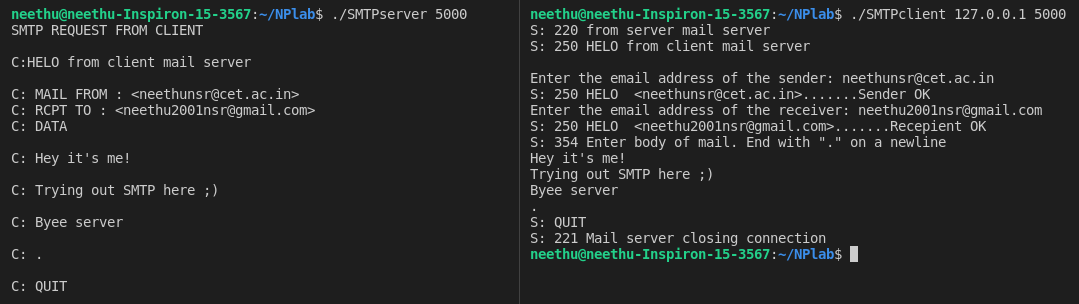
\includegraphics[scale=0.45]{img/exp11.png}
\end{figure}

\subsection{Result}
Implemented the program for the simulation of Simple Mail Transfer Protocol using UDP, using C language in Ubuntu 20.04 with kernel and the above outputs were obtained.

